%	\item Begrundelse baseret på antal op-amp / orden (6/8)
%	\item Kort teoretisk gennemgang af den valgte topologi
%	\item Beregninger og dimensionering af 6. ordens chebycheb filtre
%	\item Implementeringsvalg og design af hardware/schematics
%\end{itemize}


\section{Analoge filtres rolle ved digital signalbehandling}\label{sec:filter_intro}
\begin{wrapfigure}[30]{r}{3.5cm}
	\vspace{-.5cm}
	\centering
	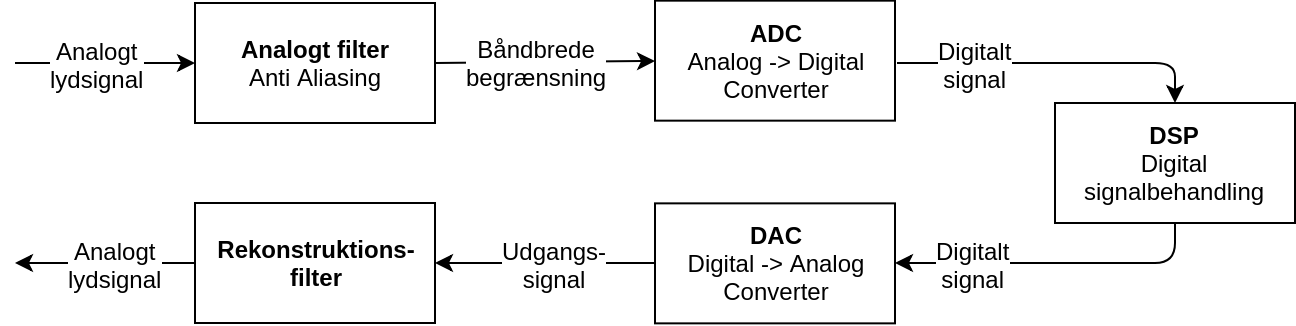
\includegraphics[width=2.5cm]{billeder/dsp_model.png}
	\caption{DSP model.}
	\label{fig:dsp_model}
\end{wrapfigure}

For at kunne udfører digital signalbehandling af et analogt signal, bliver man nød til at overfører signalet fra den analoge verden til den digitale og tilbage igen - dette sker ved sampling og rekonstruktion.
Denne signalbehandling følger nogle faste deltrin, som kan ses i et generelt signal-blok diagram i figur \ref{fig:dsp_model}.
I dette kapitel vil fokus ligge på de analoge signaler og filtre, således vil vigtigheden de analoge filtre blive kortlagt og den efterfølgende analyse og dimensionering  \\

Når et 
\jj{hvad var jeg ved at skrive her ???}

Som udgangspunkt blev opløsningen af den Analog-Digital Converter (ADC) til at vurdere hvor meget dæmpning er analogt filter skulle have for at kunne sikre en komplet og tabsfri gengivelse af signalet.

Ud fra de fremsatte krav til projektet, benyttes der en   microcontroller fra Texas Instruments \cite{spmu296} der er udstyret med en 12bit ADC på de analoge indgange.
For at bestemme opløsning på ADC'en, kan den unipolære\footnote{Unipolær kvanteficering skyldes ADC'ens spændingsområde på $0 \longmapsto \num{3.3}\si{\volt}$.} kvanteficering $\Delta_{ADC}$ bestemmes samt Signal to Noise Ratio $SNR_Q$.
   
\begin{align}
	\Delta_{ADC} &= \frac{V_{max}}{2^N} = \frac{\num{3.3}\si{\volt}}{2^{12}} \approx \num{80.6}\si{\milli\volt}\\
	SNR_Q &= 6,02 N + 2 [\si{\decibel}] = 6,02\cdot 12+2 = 74,24 \si{\decibel} 
\end{align}
 


\note{Kort teoretisk intro til hvorfor filtre skal anvendes til sampling}
\note{Båndbrede begrænsning}
\note{Shannons sampling theorem}
\note{Generel intro til audio signaler}
\note{begrundelse for orden af filter i intro}

\section{Analyse af filter typer}\label{sec:filter_analyse}
%\note{Gennem gang af de filter topologier der har været i betragtning som en mulig løsning.}
For at kunne finde frem til et passende lavpasfilter som antialiasing filter, bliver 4 tilter typer sammenlignet - Butterworth, Chebyshev type I og II samt Bessel (Thomson).
Hver af disse filtre har en tilhørende amplitudekarakteristik der beskrives med følgende overføringsfunktion\cite{anfilter}.

\begin{align} 
H_{butterworth}(j\omega_n) &= \frac{1}{\sqrt{1 + \omega_n^{2n}}} \label{eq:H_butt} \\
H_{bessel} (j\omega_n) &= \frac{H}{a_0 + \omega^2 + ja_1\omega_n} \label{eq:H_bes}\\
H_{chebychevI}(j\omega_n) &= \frac{1}{\sqrt{1 + \epsilon^2 C_n^2(\omega_n)}} \label{eq:H_cheb1} \\
H_{chebychevII}(j\omega_n) &= \frac{1}{\sqrt{1 + \frac{1}{\epsilon^2 C_n^2(\omega_n)}}} \label{eq:H_cheb2} \\
C_n(\omega_n) &=  
\begin{matrix}
	\cos(n\arccos(\omega_n)) & 0 \le \omega_n \le 1 \\  \cosh(n \arccosh(\omega_n)) & 1 \le \omega_n 
\end{matrix} \label{eq:chev_cn_funk}
\end{align}

I ligning (\ref{eq:chev_cn_funk}) fremgår den indre funktion $C_n(\omega_n)$ som bruges i Chebychev I og II i ligening (\ref{eq:H_cheb1}) og (\ref{eq:H_cheb2}).

Figur \ref{fig:filter_typer} viser en samlet fremstilling af amplitude karakteristikken $H(j\omega_n)$ og gruppeløbstiden $D(\omega_n)$ for de fire filtertyper.

\begin{figure}[h!]
	\centering
	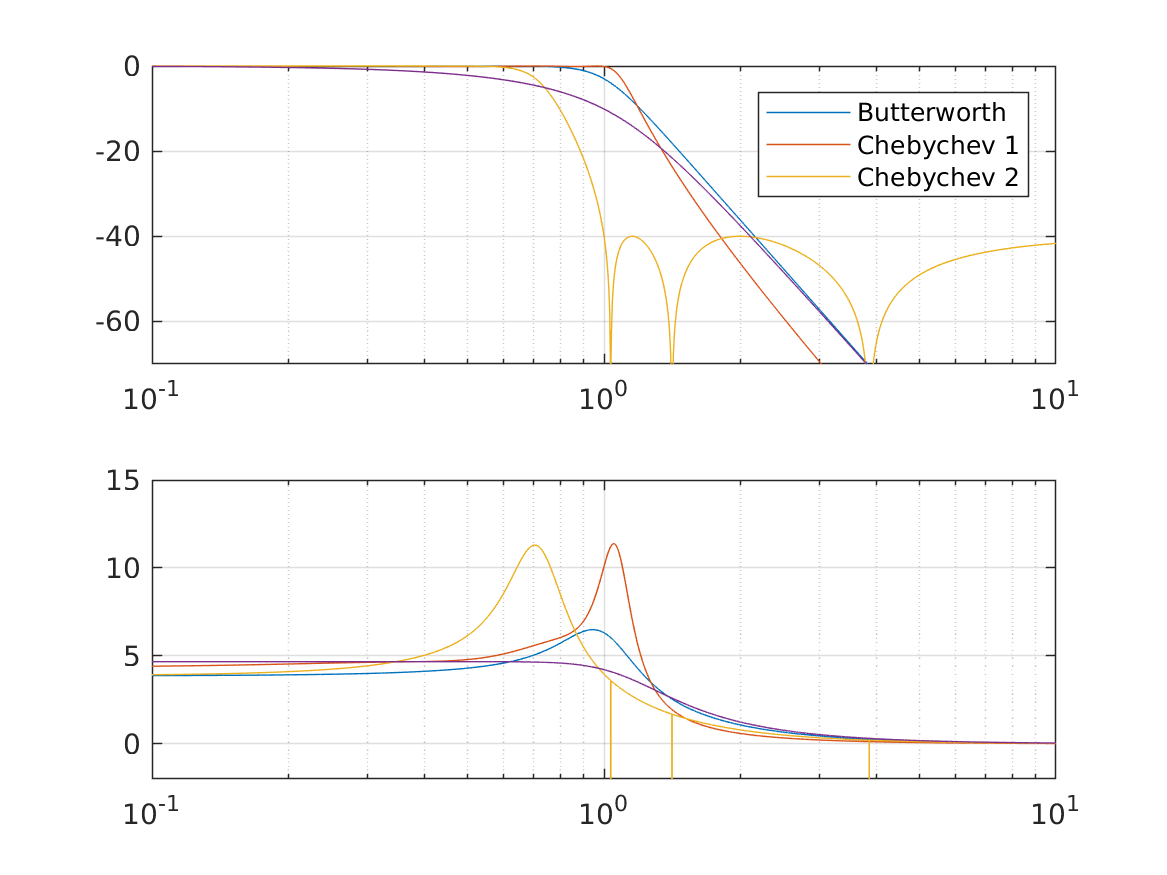
\includegraphics[width=1\textwidth]{matlab/filter_compare.png}
	\caption{Normeret 6.ordens filter karakteristik (øverst) og guppeløbstid (nederst) for filtertyperne Butterworth, Chebychev Type I ($0,1 \si{\decibel}$ rippel) \& Type II ($-40 \si{\decibel}$ stopbånds rippel) og Bessel.}
	\label{fig:filter_typer}
\end{figure}

Det ønskede filter skal have en rimelig flad karakteristisk i pasbåndet og en stejl overgang til stopbåndet.
Således kan lydsignalets amplitude holdes konstant i hele det ønskede frekvensområde da uønsket dæmpning/forstærkning af lydsignalet kan medfører hørbare ændringer af lydbilledet, på samme måde som en equalizer påvirker et lydsignal. 

Ligeledes ønskes en rimelig konstant gruppeløbetid. 
Gruppeløbetiden, der er defineret i ligning (\ref{eq:groupdelay_def})\cite{anfilter}, er et udtryk for hvor stor tidsforsinkelsen på signal som funktion af frekvensen er.

\begin{align}
	D(\omega) \stackrel{def}{=} - \dfrac{d(arg(N(\omega)))}{d\omega}\label{eq:groupdelay_def}
\end{align}

Hvis signal forsinkelsen bliver for stor i et givet frekvensområde, vil der fremstå en hørbar ændring af lydbilledet.
Dette fenomen er dog ret subjektivt og der findes mange meninger om hvilke tærskelværdier der kan accepteres.
Ud fra en lettere gennemgang inden for området, er antages en acceptabel relativ tidsforsinkelse på $D_{rel}(\omega) < -10 \si{\milli\second}$ til projektet.   

\subsection{Valg af filter topologi}
Hvis man som udgangspunkt kun fokusere på filtrenes gruppeløbstid, ville man skulle vælge et Bessel filter.
Bessel filteret, det er designet som et filter med maksimal fald fase, har dog langt fra den ønskede dæmpning i overgangsbåndet.
Det vælges at anvende et Chebychev type I filter, der viser sig at have den bedste dæmpning i overgangsbåndet.
Det høje udsving på gruppeløbetiden for denne filtertype, som det fremgår nederst i figur \ref{fig:filter_typer}, vil på det denomaliserede filter ligger indenfor, de i projektet, acceptable værdier. 
\\
I figur \ref{fig:filter_cheb1_denorm} ses den denormaliserede filterkarakteristik for det valgte filter med en pasbåndsrippel på $0,1 \si{\decibel}$ og en knækfrekvens på $f_c = 18 \si{\kilo\hertz}$. 

\begin{figure}[h!]
	\centering
	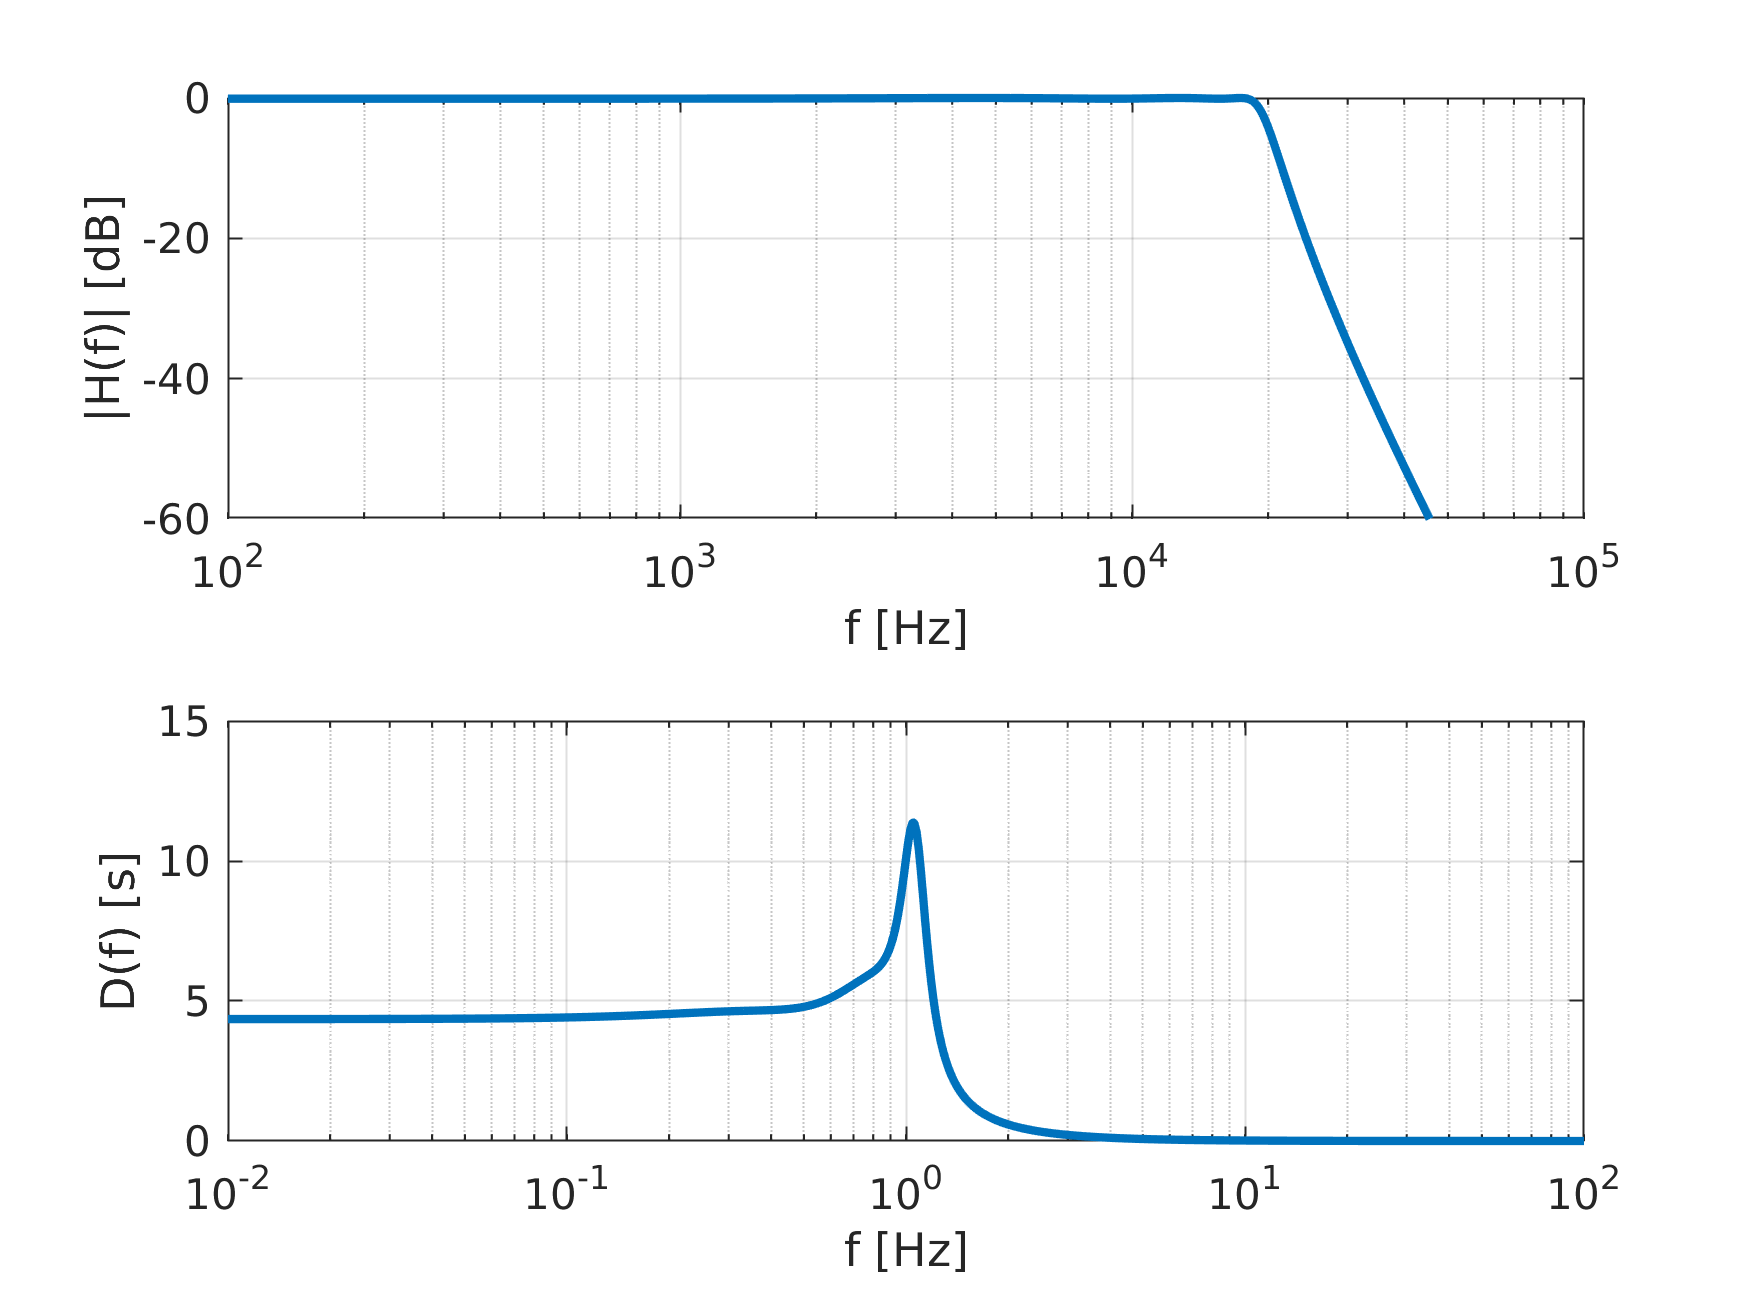
\includegraphics[width=1\textwidth]{matlab/filter_cheb1_denorm.png}
	\caption{Denormeret 6.ordens filter karakteristik og guppeløbstid af Chebyshev Type I ($0,1 \si{\decibel}$}
	\label{fig:filter_cheb1_denorm}
\end{figure}
\jj{ret matlab fil med denormineret grpdelay}

For at kunne bestemme dæmpningen af de demormaliserede filter, findes udtrykket for $|H(f)|$.
Med udgangspunkt i ligning \ref{eq:H_cheb1}, bestemmes $\epsilon$, som er bestemt ved ud fra rippelfaktoren i et Chebyshev filter\footnote{Figur 1.11.1 og ligning 1.11.3 i kilde \cite{anfilter}}
\begin{align}
	K_p = 20 \log \frac{1}{\sqrt{1+\epsilon^2}} \Leftrightarrow \epsilon = \sqrt{10^{K_p/10}-1}
\end{align}
Med en maksimal rippel på $K_p = 0,1 \si{\decibel}$ fås en $\epsilon$ på 
\begin{align}
	\epsilon = \sqrt{10^{0,1/10}-1} = \num{0.1526}
\end{align}

Da det ønskes at beregne $|H(f)|$ i området $f > f_c$ anvendes $C_n$ fra ligning \ref{eq:chev_cn_funk} hvor $w_n > 1$
Dæmpningen ved nyquistfrekvensen på $f_s/2 = \num{22.05}\si{\kilo\hertz}$ kan nu bestemmes som

\begin{align}
|H(f)|_{\si{\decibel}} &= 20 \log \frac{1}{\sqrt{1+ \epsilon^2  \left[\cosh(n \arccosh k )\right]^2 }} \quad, \quad k = \frac{f}{f_c} \\
|H(22,05\si{\kilo\hertz})|_{\si{\decibel}} &= 20 \log \frac{1}{\sqrt{1+ 0,1526^2  \left[\cosh(n \arccosh \frac{22,05\si{\kilo\hertz}}{18\si{\kilo\hertz}} )\right]^2 }} = \num{-12.2568} \si{\decibel}
\end{align}

\subsection{Forventet aliasing ved valgte filter type}
\jj{lidt mere intro til aliasing}
I figur \ref{fig:filter_f_fs} ses amplitude karakteristikken $|H(f)|$ af det valgte filter med blåt og den første periodiske gentagelse af frekvens spektrum $|H(f-f_s)|$ med rødt.
\begin{figure}[h!]
	\centering
	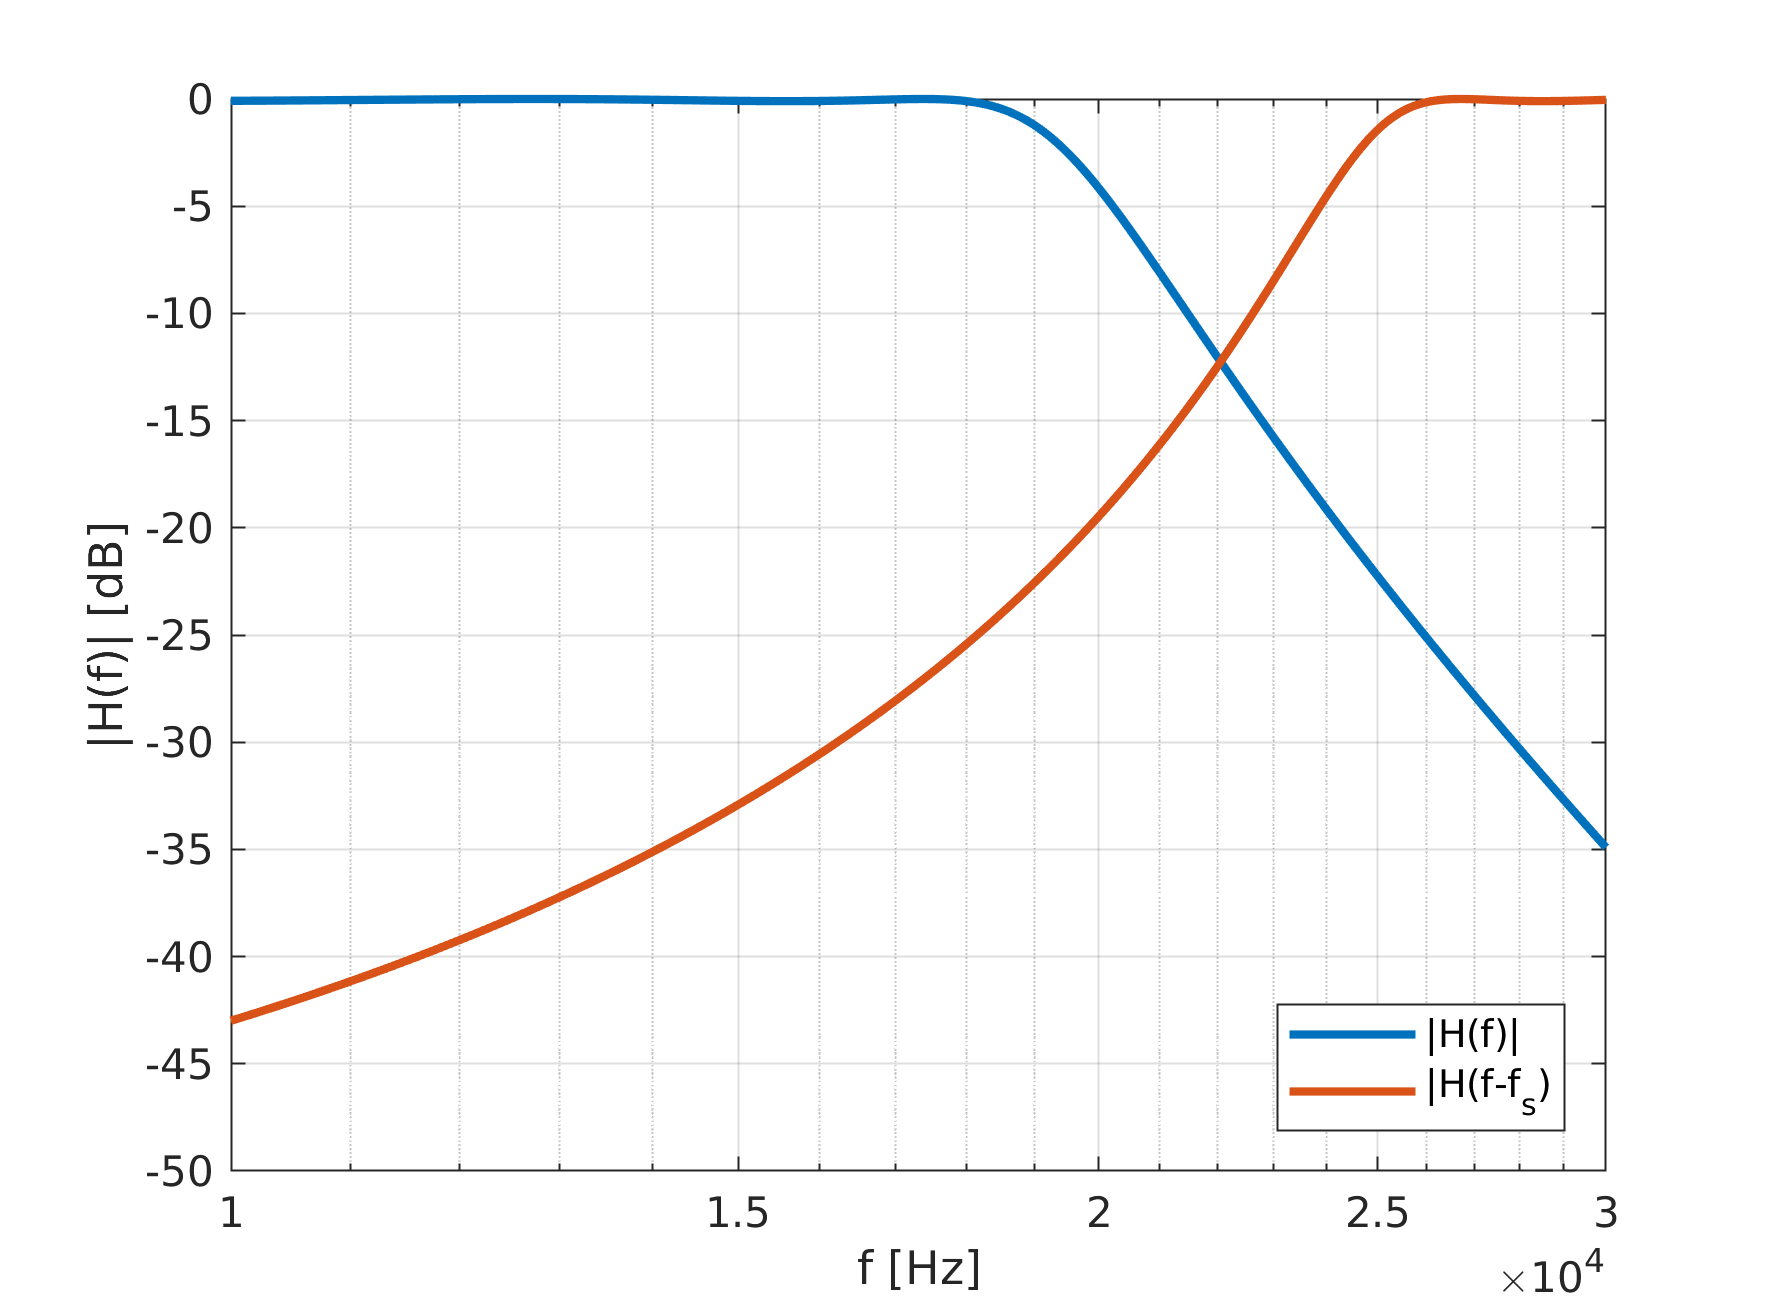
\includegraphics[width=.8\textwidth]{matlab/filter_f_fs.png}
	\caption{}
	\label{fig:filter_f_fs}
\end{figure}

En dæmpning på kun $\num{12.3} \si{\decibel}$ ved Nyquistfrekvensen er ikke ret stor og der må derfor ventes aliasing i signalet.
Størrelsen af aliasing i signalet $SA$, kan beregnes som procentvis del ved
\begin{align}
	\%SA = \frac{|H(f)|_{f=f_s-f_x}}{|H(f)|_{f=f_x}} \cdot 100 \% \label{eq:signal_alias}
\end{align} 
I ligning \ref{eq:signal_alias} angiver $f_x$ den frekvens, hvor den procentvise aliasing effekt ønskes beregnet.
Effekten kan evalueres ved at plotte $SA(f)$ fra ligning \ref{eq:signal_alias} som ses i figur \ref{fig:filter_sa}, både angivet som procentvis forhold og absolut i decibel.
Her er det således muligt at se, at der ved fx $f_c=\num{18}\si{\kilo\hertz}$ er en aliasing effekt på $5,4\%$.

\begin{figure}[h!]
	\centering
	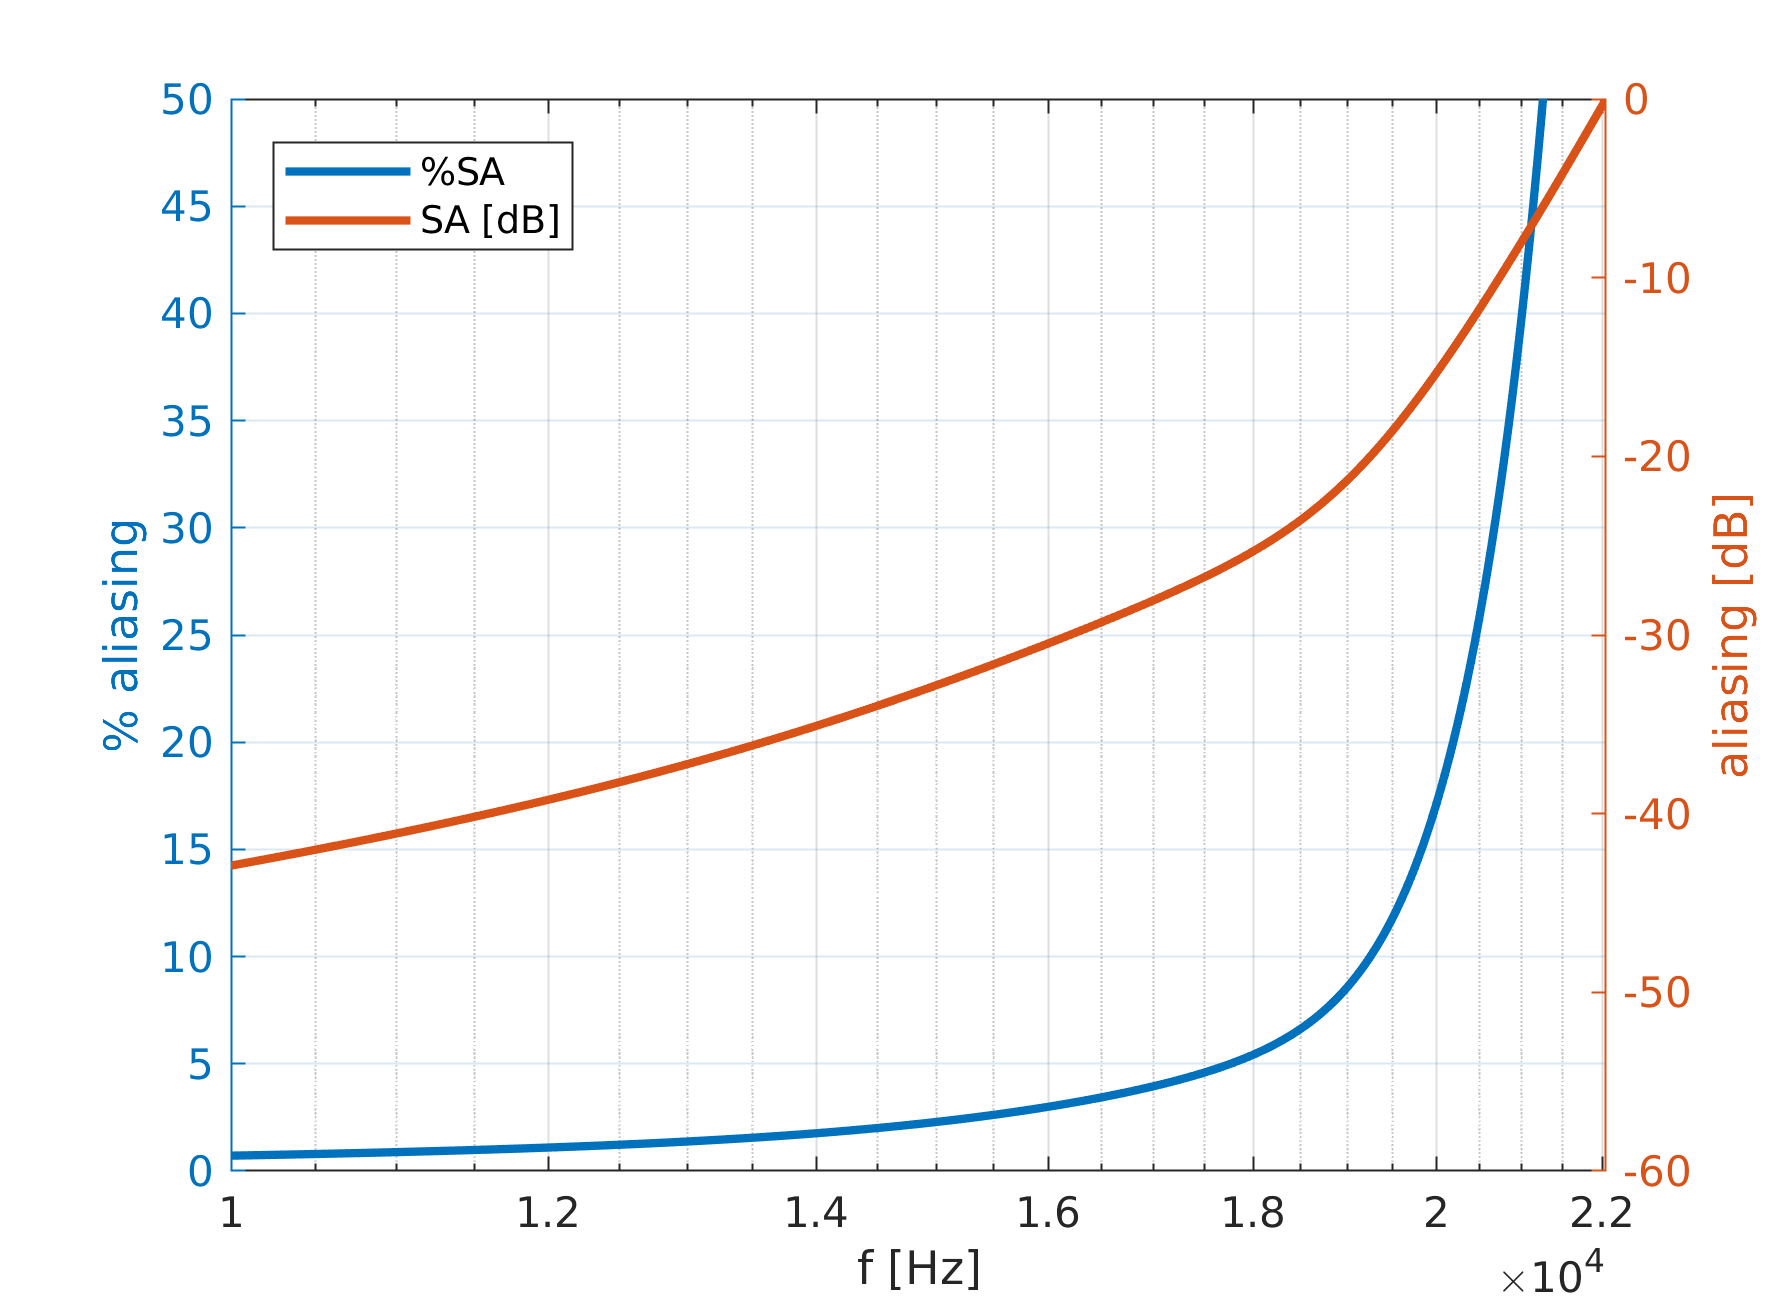
\includegraphics[width=.8\textwidth]{matlab/filter_sa.png}
	\caption{}
	\label{fig:filter_sa}
\end{figure}

%\note{Beregninger og argumentation for SNR}

\section{Specifikation og dimensionering}\label{sec:filter_spec}



\note{sprecifikation som bi-quad systemer}
\note{hvor tæt ligger de beregnede komponent værdier i hold til de anvendte tabelværdier ?}
\note{Sallen Kay - metode 4 i afs matr.}
\note{Hvordan kommer aliasing til at have indflydelse på det endelige signal ved valg af 6. ordens filter} 


\section{Design og implementering}\label{sec:filter_design}
\note{Fremstilling i bi-quad print}
\note{Argumenteret valg er OpAmp -> den bedste der var som SMD}
\note{Kort begrundelse for enkelt R i metoden og brug af op til 4 stk. C som proto type -> hvordan ville det se ud hvis kun brugte den nærmeste C i serien og hvor stor indflydelse vil det have. Måske Sensitivitesmetoden eller H(jw) -> var det er klogt valg og måske lidt overdrevet.}

\section{Rekonstruktions filter}
\note{Hvorfor anvendes et tilsvarende AA filter på udgangen - lidt teori her}

